\subsection{Visão Geral}
Este teste visou testar a aplicabilidade do sensor laser Faro Focus 3D X330 no
ambiente de trabalho da turbina. O dipositivo apresenta sensibilidade a
ambientes onde haja alta umidade, pois opera com um sistema de lentes e lasers e
caso apresente condensação em um desses componentes, o resultado final de
sensoriamento pode ser prejudicado. Por esse motivo foi necessário realizar
testes com o sistema para analisar a viabilidade técnica de se usar o sensor
para a aplicação do projeto EMMA. 


\subsection{Equipamentos utilizados}

\begin{enumerate}
\item Faro Focus 3D X330 
\item Tripé de apoio
\item Esferas Reflexivas com base magnética
\end{enumerate}

\begin{figure}[h!]
\centering
	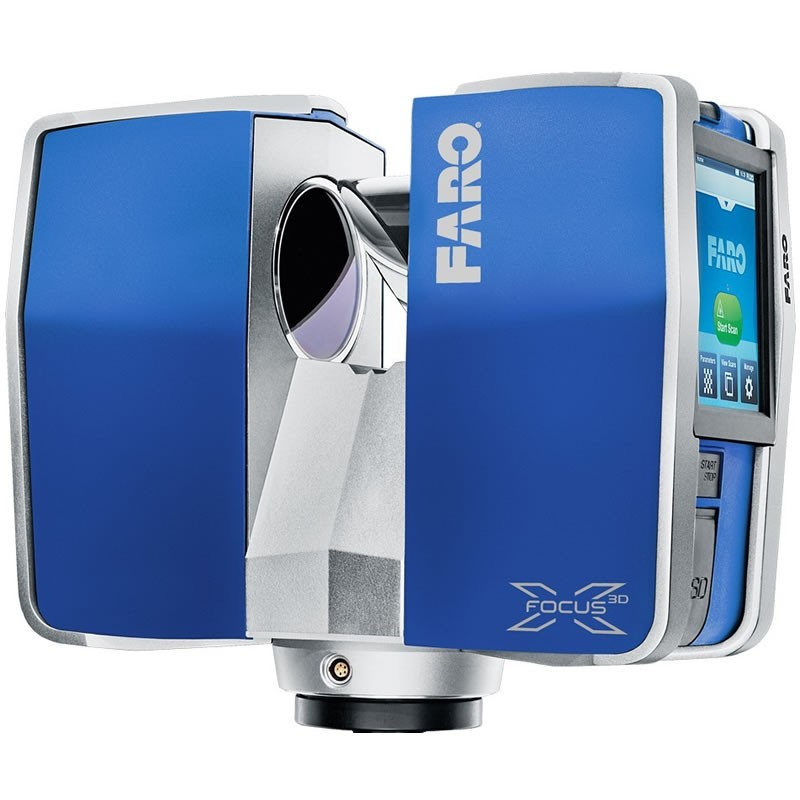
\includegraphics[width=0.4\columnwidth]{figs/faro/sensor}
	\caption{Sensor Faro Focus 3D X330.}
	\label{fig::sensor}
\end{figure}

\begin{figure}[h!]
\centering
	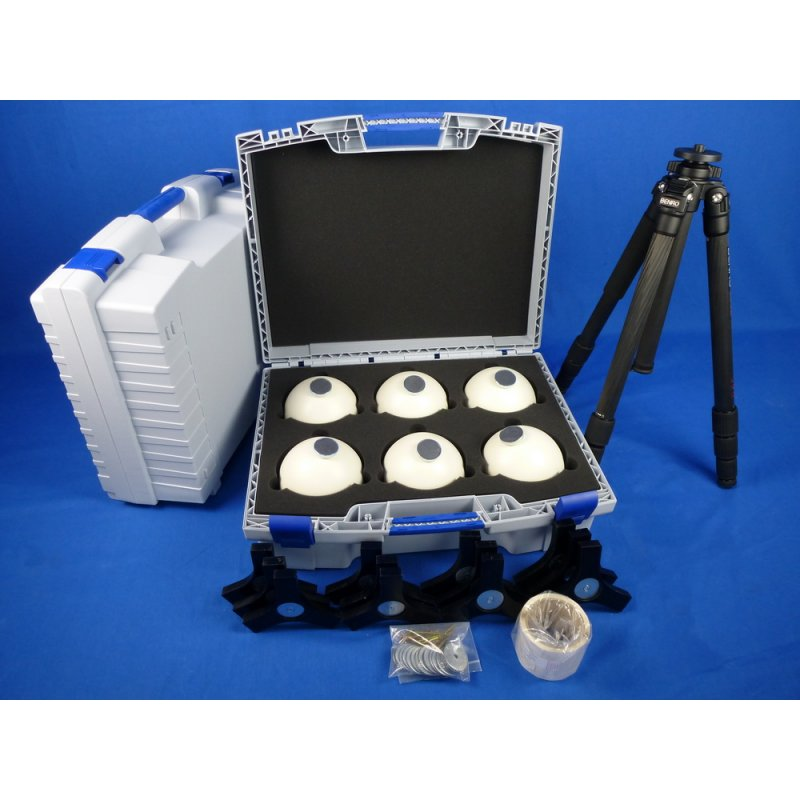
\includegraphics[width=0.5\columnwidth]{figs/faro/kit}
	\caption{Conjunto de esferas Reflexivas e tripé}
	\label{fig::kit}
\end{figure}


\subsection{Dados dos equipamentos}

\begin{itemize}
  \item Faro Focus 3D X300
  \begin{itemize}
    \item \textbf{Alcance:} 0,6 m - 330 m
    \item \textbf{Velocidade de medição (pts/seg.):}s 122.000 / 244.000 /
    488.000 / 976.000
    \item \textbf{Erro de alcance:} $\pm 2 mm$
    \item \textbf{Campo de visão vertical (vertical/horizontal):} 300$^o$ /
    360$^o$
    \item \textbf{Tamanho do passo (vertical/horizontal):} 0,009$^o$
    \item \textbf{GPS:} Receptor GPS integrados
    \item \textbf{Peso:} 5,2 kg
    \item \textbf{Temperatura ambiente:} $5^o - 40^o C$
    \item \textbf{Umidade:} Sem condensação
  \end{itemize}
\end{itemize}

\subsection{Procedimento}

\subsection{Resultados} 

\subsection{Conclusões}
